% !TeX spellcheck = de_CH
\documentclass[
a4paper,
oneside,
10pt,
fleqn,
headsepline,
toc=listofnumbered, 
bibliography=totocnumbered]{scrartcl}

% deutsche Trennmuster etc.
\usepackage[T1]{fontenc}
\usepackage[utf8]{inputenc}
\usepackage[english, ngerman]{babel} % \selectlanguage{english} if  needed
\usepackage{lmodern} % use modern latin fonts

% Custom commands
\newcommand{\AUTHOR}{M. Wieland}
\newcommand{\SECONDAUTHOR}{F. Hauser}
\newcommand{\THIRDAUTHOR}{M. Trentini}
\newcommand{\FOURTHAUTHOR}{P. Scherler}
\newcommand{\INSTITUTE}{Hochschule für Technik Rapperswil}
\newcommand{\LECTURER}{Prof. Dr. Jürg Stadelwieser}
\newcommand{\GITHUB}{https://github.com/michiwieland/businessplan}

% Jede Überschrift 1 auf neuer Seite
\let\stdsection\section
\renewcommand\section{\clearpage\stdsection}

\makeatletter
\newcommand\invisiblesection[1]{%
	\refstepcounter{section}%
	\addcontentsline{toc}{section}{\protect\numberline{\thesection}#1}%
	\sectionmark{#1}\phantom{}}
\makeatother

% Multiple Authors
\usepackage{authblk}

% Include external pdf
\usepackage{pdfpages}

% Layout / Seitenränder
\usepackage{geometry}

% Inhaltsverzeichnis
\usepackage{makeidx} 
\makeindex

\usepackage{url}
\usepackage[pdfborder={0 0 0}]{hyperref}
\usepackage[all]{hypcap}
\usepackage{hyperxmp} % for license metadata

% Glossar und Abkürzungsverzeichnis
\usepackage[acronym,toc,nopostdot]{glossaries}
\glossarystyle{altlisthypergroup}
\usepackage{xparse}
\DeclareDocumentCommand{\newdualentry}{ O{} O{} m m m m } {
	\newglossaryentry{gls-#3}{name={#5},text={#5\glsadd{#3}},
		description={#6},#1
	}
	\makeglossaries
	\newacronym[see={[Siehe:]{gls-#3}},#2]{#3}{#4}{#5\glsadd{gls-#3}}
}
\makeglossaries

% Mathematik
\usepackage{amsmath}
\usepackage{amssymb}
\usepackage{amsfonts}
\usepackage{enumitem}

% Images
\usepackage{graphicx}
\graphicspath{{images/}} % default paths

%figures
\usepackage{tikz}
\usetikzlibrary{shapes.geometric}

%risk-rating
\newcommand\risk[2]{
	\begin{tikzpicture}
	\draw [thick, |->] (0,2) -- (#2,2);
	\draw [fill=red, thick] (#1,2) circle [radius=0.2];
	\end{tikzpicture}
}

% Boxes
\usepackage{fancybox}

%Tables
\usepackage{tabu}
\usepackage{booktabs} % toprule, midrule, bottomrule
\usepackage{array} % for matrix tables

% Multi Columns
\usepackage{multicol}

% Header and footer
\usepackage{scrlayer-scrpage}
\setkomafont{pagehead}{\normalfont}
\setkomafont{pagefoot}{\normalfont}
\automark*{section}
\clearpairofpagestyles
\ihead{\headmark}
\ohead{\TITLE}
\cfoot{\pagemark}

% Pseudocode
\usepackage{algorithm}
\usepackage{algorithmic}

% Code Listings
\usepackage{listings}
\usepackage{color}
\usepackage{beramono}

\definecolor{DarkPurple}{rgb}{0.4, 0.1, 0.4}
\definecolor{DarkCyan}{rgb}{0.0, 0.5, 0.4}
\definecolor{LightLime}{rgb}{0.3, 0.5, 0.4}
\definecolor{Blue}{rgb}{0.0, 0.0, 1.0}

\lstdefinestyle{eclipse-style}{
	language=Java,
	columns=flexible,
	showstringspaces=false,
	basicstyle=\footnotesize\ttfamily, 
	keywordstyle=\bfseries\color{DarkPurple},
	commentstyle=\color{LightLime},
	stringstyle=\color{Blue}, 
	escapeinside={£}{£}, % latex scope within code
	morekeywords={length},
	numbers=left,
	numberstyle=\tiny\color{black},
	frame=single,
}
\lstset{style=eclipse-style}


% Theorems \begin{mytheo}{title}{label}
\usepackage{tcolorbox}
\tcbuselibrary{theorems}
\newtcbtheorem[number within=section]{definiton}{Definition}%
{fonttitle=\bfseries}{def}
\newtcbtheorem[number within=section]{remember}{Merke}%
{fonttitle=\bfseries}{rem}
\newtcbtheorem[number within=section]{hint}{Hinweis}%
{fonttitle=\bfseries}{hnt}

% Dokumentinformationen
\newcommand{\SUBJECT}{Businessplan}
\newcommand{\TITLE}{GitFit}

% pdf metadata
\hypersetup{
	pdfauthor={\AUTHOR},
	pdftitle={\SUBJECT \TITLE}
}

\begin{document}


% German \and
\renewcommand\Authands{ und }
% Front page
\title{\TITLE}
\subject{\SUBJECT}
\author{\SECONDAUTHOR}
\author{\THIRDAUTHOR}
\author{\FOURTHAUTHOR}
\author{\AUTHOR}
\affil{\INSTITUTE}
\affil{\LECTURER}
\date{\today}
\maketitle

\pagecolor{PrimaryColor}\afterpage{\nopagecolor}

\begin{center}
	
\includegraphics[width=0.7\linewidth]{images/front}
\end{center}


\color{black}


% Table of contents
\tableofcontents


% Glossar and acronyms (if included \loadglsentries{glossar})
\printglossary[type=\acronymtype]
\printglossary
\glsaddall


%TODO Total: 20 Seiten -> Es muss ersichtlich sein, was das Produkt bringt.
%TODO Sturktur nach PWC -> Siehe PDF auf Skripte Server

\section{Abstract}


% TODO Wir bieten flexibiltät, effizienz, komfort


\section{Das Businessmodell}
%TODO Import Canvas \includepdf[pages={1},landscape=true]{appendix/schemes/datacenter.pdf}

\section{Mission, Vision und Strategie: die Zukunft}
\subsection{Mission}
Unsere Aufgabe ist es, vielen Menschen ein völlig neues Erlebnis für ein persönliches Training im Fitnesscenter zu bieten. Wir tun dies, indem wir eine App anbieten, welche die Fitnesslandschaft revolutioniert. Dies zu Preisen, die sich auch kleine Fitnesscenter leisten können.

\subsection{Vision}
Schweizer Fitnesscenter setzen aktuell vorzugsweise auf Papier und Bleistift für die Trainingsplanung ihrer Kunden. Dies ist nicht mehr zeitgemäss und bedarf einer Generalüberholung. Am Puls der Zeit zu sein, bedeutet für ein Fitnesscenter, einen modernen und attraktiven Dienstleister für seine Kunden darzustellen. Die Digitalisierung bietet unendlich viele Möglichkeiten, die es zu nutzen gilt. \\
Wir wollen eine App kreieren, welche die Fitnessbranche wieder auf den aktuellen Stand der Technik katapultiert. Die App bietet aufschlussreiche Statistiken sowie hilfreiche Tipps zur Übung, wenn der Trainer gerade nicht in der Nähe ist.

\subsection{Strategie}
Unser Angebot richtet sich in erster Linie an grosse Fitnesscenter-Ketten, da wir glauben, dass diese an einem übergreifenden Wissensaustausch der Filialen interessiert sind. Im Rahmen der Entwicklung kümmern wir uns in einer ersten Phase um das Anreichern von Stammdaten mit auserwählten Partner-Center. Die Daten sollen als solides und realitätsnahes Fundament für die weitere Entwicklung dienen. In einer zweiten Phase wird dann die App für den Endkunden entwickelt, die ein möglichst komfortables und persönliches Trainingserlebnis vermitteln soll. 

\subsubsection{Wettbewerbsstrategie}
Der Schweizer Fitnessmark boomt und trotzdem ist keine Digitalisierung in der Branche erkennbar. Ähnliche Projekte finden im Ausland bereits Anklang, jedoch gibt es im Inland keine vergleichbare Dienstleistung. Grund genug, diese Lücke zu füllen. Die Schwierigkeit in dem Projekt liegt deshalb weniger in der Positionierung gegenüber ausländischen Dienstleister, sondern vielmehr die heimischen Fitnesscenter mit der neuen Technologie vertraut zu machen.


\section{Produkte und Dienstleistungen: die Marktleistung}

\subsection{Die App}
\begin{figure}[h]
\centering
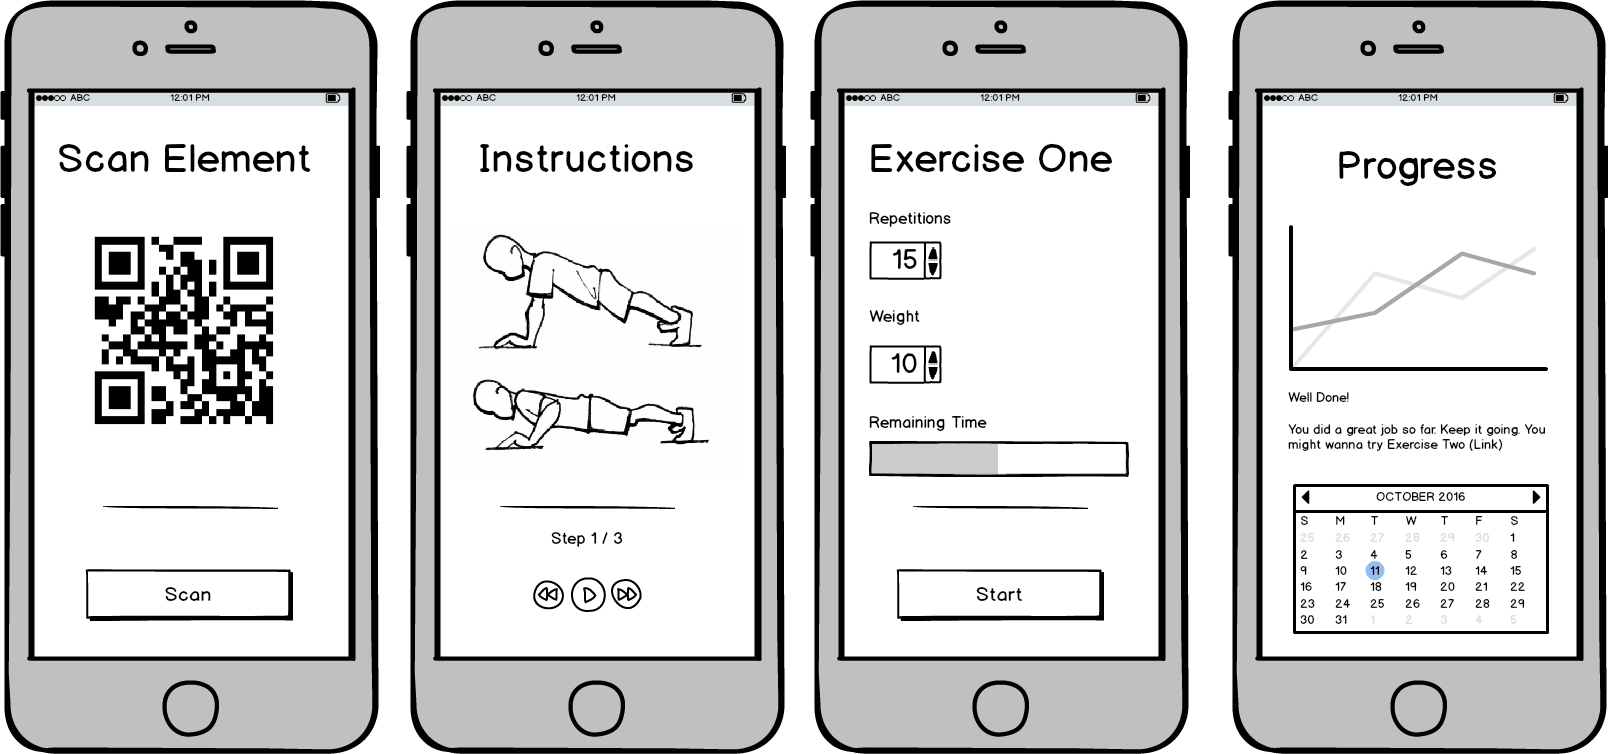
\includegraphics[width=0.5\linewidth]{images/app}
\caption{Wireframe der App}
\label{fig:app}
\end{figure}


\section{Markt und Kunden: das Zielgebiet}

\section{Konkurrenz: die Mitbewerber}
Auf dem schweizer Markt ist die Konkurrenz noch eher klein. Erst wenige Fitnesscenter haben sich selber oder wurden von einem Dienstleister digitalisiert. Jedoch gibt es einige Anbieter im nahen Ausland, für welche die Schweiz einen attraktiven Mark bietet. Beide Gruppen wollen wir als potentielle Konkurrenten analysieren.
\paragraph{myClubs}\hfill \\
myClubs\cite{myclubs} ist ein schweizer Anbieter einer Fitness App. Ihr Ziel ist es, einem Sportler eine flexible Möglichkeit zu bieten Sport zu treiben. Dabei legen sie ihren Fokus jedoch nicht darauf Fitnesscenter attraktiver zu gestalten oder zu digitalisieren, sondern dem Sportler ein breites Sportangebot in einem einzigen Abo zu bieten. Endkunden von myClub sind also Sportler.
Das myClubs Angebot umfasst:
\begin{itemize}
	\item Auswahl an verschiedenen Sportarten und -kursen
	\item Auswahl an verschiedenen Partner-Anbietern
	\item Zum Fixpreis im Abosystem
\end{itemize}
Wir heben uns vom Konkurrenten myClub ab, da wir unseren Fokus auf die Verbesserung des Kraft- und Ausdauertrainings in einem Fitnesscenter legen.
\paragraph{eGym}\hfill \\
Der deutsche Anbieter eGym\cite{egym} verfolgt sehr ähnliche Ziele wie wir. Sie bieten ihren Partnerfitnesscentern eine App mit folgenden Kernfunktionen:
\begin{itemize}
	\item Zugriff auf den Trainingsplan des Fitnesstrainers
	\item Dokumentation von Trainingseinheiten
	\item Kontrolle über Trainingserfolg und Vergleich mit Kollegen
\end{itemize}
eGym wäre ein starker potentieller Konkurrent, falls er in den schweizer Markt expandieren würde.
%TODO: Konkrete Abgrenzung?
\paragraph{Technogym}\hfill \\
Technogym\cite{technogym}ist ein Anbieter aus der Niederlande. Sie bewegen sich im selben Marktsegment wie wir. Sie verkaufen ihre Fitnessapp sowie angebundene Fitnessgeräte an ihre Fitnesscenter-Kunden.
Ihre Produktpalette umfasst:
\begin{itemize}
	\item Fitnessgeräte mit digitalen Funktionen
	\item vom Trainer erstellte Fitnesspläne mit der Prescribe-App
\end{itemize}
%TODO: Konkrete Abgrenzung?
\paragraph{Freeletics}\hfill \\
Der deutsche Dienstleister Freeletics\cite{freeletics} entwickelt eine eigene Fitness-App und betreibt eine Fitnesscenter-Kette.
Folgendes Angebot bietet Freeletics:
\begin{itemize}
	\item App mit Übungsanleitungen und Fortschrittstracking
	\item Ihre eigene Fitnesscenter-Kette
\end{itemize}
Da Freeletics ihre eigene Fitnesscenter-Kette betreibt, wären sie nur dann ein ernsthafter Konkurrent, wenn sie in die Schweiz expandieren und hier ansässige Fitnesscenter vom Markt vertreiben.

\subsection{Konkurrenzanalyse}
\begin{figure}[h]
\centering
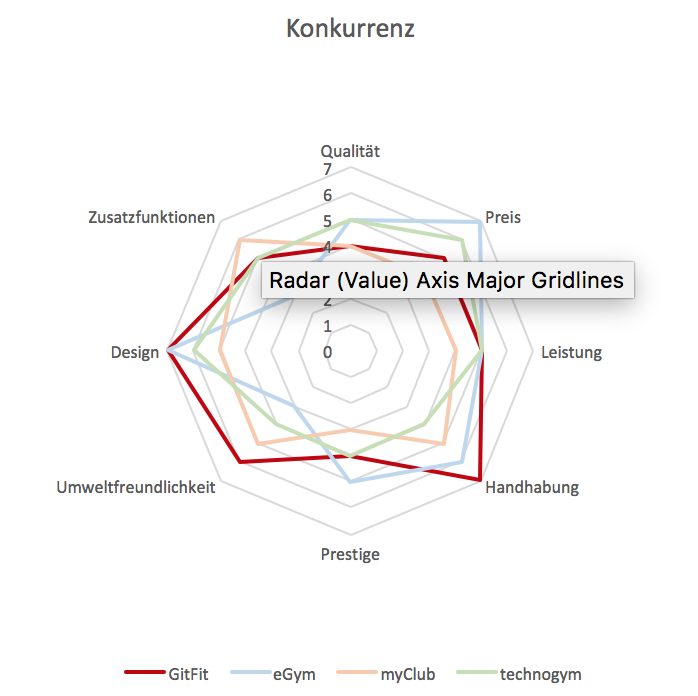
\includegraphics[width=0.7\linewidth]{images/konkurrenz}
\caption{Konkurrenzanalyse}
\label{fig:konkurrenz}
\end{figure}

\section{Marketing: der Weg zum Markt}

\subsection{Marktpositionierung}
Wir setzen primär auf den Schweizer Mark, wobei wir uns darauf konzentrieren, eine grosse Fitnesscenter-Kette als Partner zu gewinnen. Da die Branche von wenigen ''Big Player'' dominiert wird,  wird sich deren Einsatz von GitFit bei den Konkurrenzlinien und kleineren Fitnesscenter herumsprechen. Fitnesscenter die noch auf herkömmliche Arbeitsmethoden setzen, werden als nicht mehr zeitgemäss betrachtet und so zu einer Digitalisierung gezwungen. Wir unterscheiden zwischen zwei Typen von Fitnesscenter die als Kunden in Frage kommen.

\paragraph{Fitnesscenter Ketten} \hfill \\
Die grossen Fitnesscenter-Ketten sind besonders am übergreifenden Wissensaustausch ihrer regionalen Niederlassungen interessiert. So können Trainingspläne von einem Trainer Komitee erstellt werden und national in den verschiedenen Fitnesscenter auf ihre Praktikabilität überprüft werden. Entsprechende Anpassungen wirken sich auf alle beteiligten Fitnesscenter aus. Ebenfalls herrscht eine grosse Konkurrenz zwischen den einzelnen Ketten. Sich abzuheben scheint immer wie schwieriger und deshalb ist GitFit ein willkommenes Produkt zur eigenen Hervorhebung im Markt. 

\paragraph{Kleinere private Fitnesscenter} \hfill \\
Die kleineren, meist privat geführten Fitnesscenter, sind an einer kostengünstigen Lösung interessiert, um nicht an Attraktivität gegenüber den ''Big Player'' zu verlieren und Schritt zu halten. 

\subsection{Preispolitik}
\subsubsection{Preisfindung}
GitFit wird als Abomodell angeboten, wobei die Abokosten monatlich entrichtet werden müssen. Dies erlaubt es bei insolventen Kunden schnell und unkompliziert die Partnerschaft aufzulösen. 

\subsubsection{Preisdifferenzierung}
Den Fitnesscenter wird eine Plattform geboten, über welche sie die komplette Trainingsplanung selbständig durchführen können. Dank einer intuitiven Oberfläche entsteht kein Mehraufwand gegenüber der herkömmlichen Lösung mittels Stift und Papier. Der Mehrwert 

%TODO wie können wir günster sein wie unsere Konkurrenz? Vergleich mit Konkurenz absatz

\subsubsection{Rabatte}
Die App basiert auf Praxis erprobten Stammdaten die in einer ersten Phasen mit auserwählten Partnerorganisation aufgebaut werden sollen. Teilnehmende Fitnesscenter profitieren von einer vergünstigten Dienstleistung im ersten Jahr sowie dem Vorteil einer aktiven Mitgestaltung des finalen Produktes.


\subsection{Distribution}
Gerade am Anfang des Produkt soll eine enge Bindung zwischen der Entwicklung und den beteiligten Fitnesscenter bestehen. Für die Bekanntmachung unserer Dienstleistung setzen wir auf verschiedenen Distributionspfade. 

\paragraph{Produktpräsentationen}
Als kleines Startup gehen wir persönlich bei auserwählten Fitnesscenter vorbei und stellen den Nutzen unserer Plattform im persönlichen Gespräch vor. Wir suchen nach einem Partner, der uns auch auf persönlicher und nicht nur finanzieller Ebene entspricht, und die Ideologie mit uns teilt. 

\paragraph{Homepage} \hfill \\
Nach einer Evaluierungsphase soll sich auch der Endkunde (Sportler) auf unserer Homepage über das eingesetzte Produkt und dessen Vorteile informieren können. Die Homepage orientiert sich an zwei Zielgruppen. Einerseits soll es dem Endkunden genügend Infos über die App und deren Vorteile bieten und andererseits den Fitnesscenter eine Möglichkeit geben mit uns in Kontakt zu treten. Der Kunde (Fitnesscenter) soll bereits auf der Homepage ein Gefühl vermittelt kriegen, in welchem er sich betreut fühlt und einer Partnerschaft positiv entgegengestellt ist.  

\paragraph{Schulungen} \hfill \\
Hat das Produkt im Markt Fuss gefasst, gilt es die Position zu stärken. Dies wird mit motivierten Trainer erledigt, die das Personal des Fitnessstudio für den Einsatz von GitFit schult.

\subsection{Werbung und Public Relations}
In erster Linie muss ein passendes Fitnesscenter gefunden werden. Dies ist vorzugsweise eine grosse Ketten mit national verteilten Niederlassungen und einem breiten Kundenstamm. Ist ein solcher gefunden, kann über den Verband und Krankenkassen gezielt Werbung für das neue Produkt lanciert werden. 

\subsubsection{Angestrebtes Image}
GitFit ist ein innovatives, zukunftsweisendes Startup, das die Fitnessbranche revolutioniert. Fitnesscenter die GitFit unterstützen, werden als modern und attraktiv angesehen. Der Einsatz von GitFit bedeutet für ein Fitnesscenter mehr Kunden, die aus den Möglichkeiten der App, den optimalen Nutzen für ihre Gesundheit ziehen möchten.

\subsubsection{Werbeanstrengungen}
Mit einem prestigeträchtigen Partner, lässt sich Werbung vergleichsweise kostengünstig bewältigen. Die grössten Anstrengungen liegen in der Suche eines solchen Partners. Dazu setzen wir uns mit dem Verband der Schweizerischen Fitness- und Gesundheitscenter (SFGV) und den grössten Fitnesscenter-Ketten zusammen. Diesen soll der Nutzen von GitFit vorgeführt werden. Ein weiterer Vertriebskanal können Fachzeitschriften sein, die in vielen Fitnesscenter aufliegen.

\subsection{Absatzziele}
Ziel ist es, alle grossen Fitnesscenter-Ketten in der Schweiz mit GitFit auszurüsten. Ist dies geschafft können umfassende Statistiken erstellt werden, die man z.B wieder in die Forschung einfliessen lassen kann und z.B für Krankenkassen interessant sein könnte. Natürlich wäre diese Dienstleistung nicht kostenlos und bedarf einer neuen Evaluierung. Da dies aber ein erfolgreiche Platzierung im Mark voraussetzt, wird dieser Schritt hier nicht mehr weiter erörtert.

\section{Beschaffung und Produktion: die Leistungserstellung}

\section{Management und Organisation: die Köpfe dahinter}

\section{Chancen und Risiken: eine ehrliche Bilanz}

\section{Finanzieller Teil: die nackten Zahlen}
% TODO ZKB KMU Check verwenden
% Das Finanzplanungstool der ZKB muss verwendet werden!
% Investitionsplan für 3 Jahre
% Eröffnungsbilanz + Planbilanzen (3 Jahre) + Planerfolgsrechnungen (3 Jahre) (nur normal case)
% Liquiditätsplan nur für erstes Jahr (pro Monat ausgewiesen)
% Mengengerüst, das den Berechnungen zugrunde liegt.

% TODO Was ist der Kunde bereit zu zahlen?

\section{Umsetzungsplan: die Realisierung}
Musste nicht bearbeitet werden

\section{Latex Syntax}
\subsection{Untersektion}
\subsubsection{Unter Untersektion}
\paragraph{Paragraph (wird eher selten verwendet)} 

\footnote{\url{www.google.ch}}

% Ich bin ein Kommentar
% TODO Ich bin ein TODO

\begin{itemize}
	\item Bullet Point 1 
	\item Bullet Point 2
	\item Bullet Point 3
\end{itemize}

\begin{enumerate}
	\item Zahlen 1
	\item Zahlen 2
\end{enumerate}

\begin{description}
	\item[Begriff] Beschreibung
	\item[Begriff 2] Beschreibung
\end{description}

\paragraph{Mathematische Formel}
\[
	c^2 = \frac{a}{b} \cdot f
\]


\begin{table}[h]
	\centering
	\begin{tabu} to \linewidth {l l l}
		\toprule 
		1 Spalte & 2 Spalte  & 3 Spalte \\
		\midrule
		1 Spalte & 2 Spalte & 3 Spalte \\
		1 Spalte & 2 Spalte & 3 Spalte \\
		\bottomrule 
	\end{tabu} 
	\caption{Ich bin die Beschreibung einer Tabelle}
\end{table}

\begin{table}[h]
	\centering
	\begin{tabu} to \linewidth {l X}
		\toprule 
		1 Spalte  & 3 Spalte \\
		\midrule
		1 Spalte & X sollte verwendet werden, wenn wir sehr sehr sehr sehr sehr sehr sehr sehr sehr sehr sehr sehr sehr sehr sehr sehr sehr sehr sehr sehr sehr lange Zeilen haben \\
		\bottomrule 
	\end{tabu} 
	\caption{Tabelle mit Autmatischen Umbrüchen.}
\end{table}



\clearpage
\appendix

% List of figures
\listoffigures

% List of tables
\listoftables

% Bibliography
\bibliographystyle{plain} 
\bibliography{literatur}

\end{document}